\documentclass[border=8pt,12pt]{standalone}
\usepackage{times}
\usepackage{roboto}
\usepackage{inconsolata}
\usepackage[T1]{fontenc}
\usepackage{listings,xcolor}
\usepackage{tikz}
\usetikzlibrary{shadows}
\lstset{basicstyle=\ttfamily,columns=fullflexible,keepspaces=true,aboveskip=0pt,belowskip=0pt}
\begin{document}
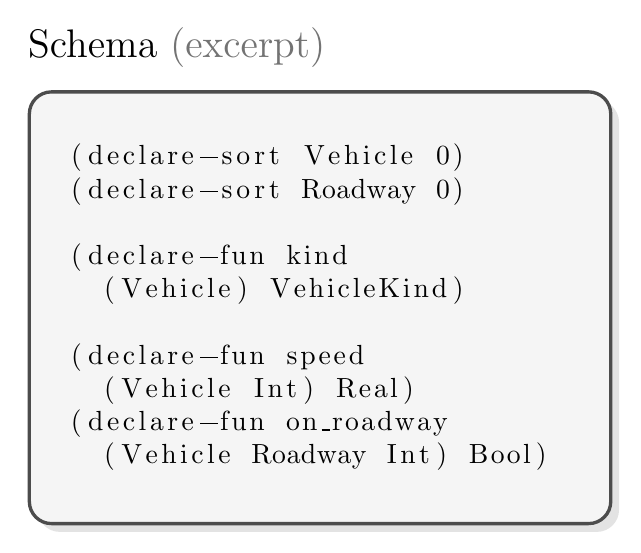
\begin{tikzpicture}
\node[draw=black!70, line width=1.2pt, rounded corners=8pt, fill=black!4, inner xsep=14pt, inner ysep=12pt,
      drop shadow={opacity=0.22, shadow xshift=3pt, shadow yshift=-3pt}] (box) {%
\begin{minipage}{6.4cm}
\begin{lstlisting}
(declare-sort Vehicle 0)
(declare-sort Roadway 0)

(declare-fun kind
  (Vehicle) VehicleKind)

(declare-fun speed
  (Vehicle Int) Real)
(declare-fun on_roadway
  (Vehicle Roadway Int) Bool)
\end{lstlisting}
\end{minipage}};
\node[anchor=south west, inner sep=0pt] at ([yshift=8pt]box.north west) {{\robotoslab\fontseries{l}\selectfont\Large Schema \textcolor{black!55}{(excerpt)}}};
\end{tikzpicture}
\end{document}
